%************************************************
\chapter{Advantages and limitations of the proposed methods}\label{ch:limitations}
In the presented thesis, we have summarized some molecular background and biological functions of nucleic acids, especially \acp{ncRNA}. Because of the implication of the secondary structure of \acp{ncRNA} in performing biological functions and the separation of the folding time scale, our study focuses on the secondary structure of \acp{ncRNA}. Therefore, we have introduced the concepts of \ac{RNA} bioinformatics and the essential computational problems related to the secondary structure of \acp{ncRNA}, such as \ac{RNA} folding and the inverse folding. We presented a comprehensive literature review on existing tools that deal with both problems and some limitations for each tool. Despite advanced field results, we have introduced two new computation tools: \texttt{RAFFT} and \texttt{aRNAque}. What are the advantages and limitations of those tools? Is there any room for further improvements? How do these tools relate to evolutionary dynamics? In this concluding chapter, we will try to provide an answer to these questions by first discussing the advantages and the limitations of the tools previously introduced. 

\section{\texttt{RAFFT}: Limitations and future works }

We presented in \autoref{ch:rafft}, \texttt{RAFFT}, a computational tool that efficiently predicts \ac{RNA} folding pathways. \texttt{RAFFT} takes advantage of the \ac{FFT} to reduce its mean computational time to $O(N^2)$, especially for long \ac{RNA} sequences (length $\geq 10^3$). We assessed \texttt{RAFFT} performance for both the secondary structure prediction task and the \ac{RNA} kinetics. In both cases, \texttt{RAFFT} shows important improvements. However, \texttt{RAFFT} also presents some limitations that will be addressed in the following section. We also discuss in this section some further improvements and applications.
 
To first assess \texttt{RAFFT} performance for the folding task, two structure estimates were compared with our method: the thermodynamic-based tools computed using \texttt{RNAfold}, \texttt{LinearFold}, \texttt{RNAstructure} and the \ac{ML} estimate using \texttt{MxFold2} and \texttt{CONTRAfold}. When we considered the lowest energy structure, the comparison of \texttt{RAFFT} to existing tools confirmed the overall validity of our approach. In more detail, a comparison with thermodynamic/\ac{ML} models yielded the following results. First, the \ac{ML} predictions performed consistently better than both \texttt{RAFFT} and other approaches, where the \ac{PPV} $=70.4\%$ and sensitivity $=77.1\%$ on average. Second, the \ac{ML} methods produced loops, such as long hairpins or external loops. We argue that the density of those loops correlates with the ones in the benchmark dataset, which a \ac{PCA} analysis revealed too.

In contrast, the density of similar loops was lower in the structure spaces produced by \texttt{RAFFT} and other thermodynamic-based methods, implying some over-fitting in the \ac{ML} model. Finally, known structures obtained through covariation analysis reflect \textit{in vivo} structure conditions. Therefore, the structures predicted by \ac{ML} methods may result from their sequences alone and their molecular environment, e.g. chaperones. We expect the thermodynamic methods to provide a more robust framework for studying sequence-to-structure relations.
Concerning thermodynamic-based tools, we obtained a substantial gain of performance when analyzing \(N=50\) predicted structures per sequence, not only the lowest energy one. This gain was even more remarkable for sequences with fewer than $200$ nucleotides, reaching the accuracy of \ac{ML} predictions. 

So how does \texttt{RAFFT} predictions contain structures that are more relevant than the \ac{MFE}, although these structures are less thermodynamically stable? The interplay of three effects may explain this finding. First, the \ac{MFE} structure may not be relevant because active structures can be in kinetic traps. Second, \texttt{RAFFT} forms a set of pathways that cover the free energy landscape until they reach local minima, yielding multiple long-lived structures accessible from the unfolded state. Third, the energy function is not perfect, so that the \ac{MFE} structures computed by minimizing it may not in fact be the most stable. 

We also showed that the fast-folding graph produced by \texttt{RAFFT} can be used to reproduce state-of-the-art kinetics, at least qualitatively. Our method demonstrated three main benefits. First, the kinetics can be drawn from as few as $68$ structures, whereas the barrier tree may require millions. Second, the kinetics ansatz describes the complete folding mechanism starting from the unfolded state. Third, for the length range tested here, the procedure did not require any additional coarse-graining into basins. (Longer \acp{RNA} might require such a coarse-graining step, in which structures connected in the fast-folding graph are merged together).

Based on our results, we believe that the proposed method is a robust heuristic for structure prediction and folding dynamics. The folding landscape depicted by \texttt{RAFFT} was designed to follow the kinetic partitioning mechanism, where multiple folding pathways span the folding landscape. This approach has shown good predictive potential. Furthermore, we derived a kinetic ansatz from the fast-folding graph to model the slow part of the folding dynamics. It was shown to approximate the usual kinetics framework qualitatively, although using significantly fewer structures. 

However, further improvements and extensions of the algorithm may be investigated. First, the choice of stems is limited to the largest in each positional lag, a greedy choice which may not be optimal. Second, we have constructed parallel pathways leading to diverse, accessible structures. Still, we have not given any thermodynamic-based criterion to identify which are more likely to resemble the native structure. We suggest using an \ac{ML}-optimized score to this effect. 

Our method can also find applications in \ac{RNA} design, where the design procedure could start with identifying long-lived intermediates and using them as target structures. We also believe that mirror encoding can be helpful in phylogenetic analysis. Indeed, the correlation spectra \(\text{cor}(k)\) computed here contained global information of base-pairing that can be used as a similarity measure. 


Finally, the versatile method implemented in \texttt{RAFFT} gives possibilities for an alternative application of the \ac{FFT} in \ac{RNA}-\ac{RNA} interaction. The underlying idea is that instead of encoding a sequence $X$ and its mirror sequence $\bar{X}$, one can consider two encoded sequences $X$ and $Y$, and the correlation between them will allow identifying the fraction of high interaction between two \ac{RNA} sequences quickly. In general, \ac{RNA}-\ac{RNA} interaction prediction methods are divided into three groups: alignment like methods, \ac{MFE} methods and comparative methods. \ac{MFE} methods constitute the majority of the \ac{RNA}-\ac{RNA} interaction tools, with the only difference often based on whether the method considers intramolecular interactions. Some methods measure the accessibility of binding region (Intra and inter interactions) \cite{umu2017comprehensive, dieterich2013computational, backofen2010computational}. We suggest neglecting intramolecular interactions and intermolecular binding pairs for a preliminary implementation. 

In sum, \texttt{RAFFT} provides a versatile framework in which the kinetic partitioning mechanism can be simulated. Therefore, it allows for predicting an ensemble of concurrent \ac{RNA} folding pathways ending in different metastable conformations. This result contrasts traditional thermodynamics techniques that find a single \ac{MFE} structure. However, further improvements of \texttt{RAFFT} could be investigated: 

\begin{itemize}
	\item The limitation of the choice of stems to the largest one in each positional lag is a greedy choice that may not be optimal. We propose to add stochastic noises in the choice of positional lag, such that running multiple times \texttt{RAFFT}, one can overcome some greediness bottlenecks.
	
	\item Our method constructs parallel pathways leading to a diverse set of
	accessible structures. Still, we have not given any thermodynamic-based criterion to identify which are more likely to resemble the native structure. We suggest using an \ac{ML}-optimized score to investigate the restrained ensemble of structures predicted by \texttt{RAFFT}.
	\item Sructures connected in the parallel pathways are separated by the
	formation or unfolding of a single stem. As mentioned above, \texttt{RAFFT} does not account for barriers between structures that stem formation could involve. Therefore, we propose to apply a post-treatment on the folding graph, where the folding path between structures is investigated using the set of valid atomic folding moves (\textit{e.g.} individual base-pair formation).
\end{itemize}

In addition to these possible improvements, we presented two possible applications: \ac{RNA} design and \ac{RNA}-\ac{RNA} interactions. In \autoref{sec:evolution}, we discuss another application in the study of evolutionary dynamics.
\section{\texttt{aRNAque}: Limitations and perspectives}
We have provided in \autoref{ch:arnaque}, a new tool \texttt{aRNAque},  implementing an \ac{EA} with a Lévy flight mutation scheme that supports pseudoknottted \ac{RNA} secondary structures. We discuss in this section the advantages of using \texttt{aRNAque} for \ac{RNA} design and some limitations that could be addressed for further improvements.

The Lévy mutation scheme offered exploration at different scales (mostly local search combined with rare big jumps). Such a scheme significantly improved the number of evaluations needed to hit the target structure, while better avoiding getting trapped in local optima. The benefit of a Lévy flight over a purely local  mutation search allowed us to explore \ac{RNA} sequence space at all scales. Such a heavy tailed distribution in the number of point mutations permitted the design of more diversified sequences. The main advantage of using a Lévy flight over local search was more remarkable for the pseudoknotted \ac{RNA} targets, which is a reduction in the number of generations required to reach a target (see \autoref{Fig:OP_vs_aRNAque}). This is because the infrequent occurrence of a high number of mutations allow a diverse set of sequences among early generations, without the loss of robust local search. One consequence is a rapid increase in the population mean fitness over time and a rapid convergence to the target of the maximally fit sequence. To illustrate that advantage, we ran \texttt{aRNAque} starting from an initial population of unfolded sequences, both for a "one point mutation" and "Lévy mutation".

 \autoref{Fig:diversity}A and  \autoref{Fig:diversity}B show respectively the max/mean fitness over time and the number of distinct structures discovered over time plotted against the number of distinct sequences. When using a Lévy mutation scheme, the mean fitness increases faster in the beginning but stays lower than that using local mutations. Later in the optimisation, a big jump or high mutation on the \ac{RNA} sequences produces structures with fewer similarities and, by consequence, worse fitness. In the $(5-10)^{th}$ generation, sequences folding into the target are already present in the Lévy flight population, but only at the $30^{th}$ generation are similar sequences present in the local search population. The Lévy flight also allows exploration of both the structure and sequence spaces, providing a higher diversity of structures for any given set of sequences (\autoref{Fig:diversity}B). Using the mean entropy of structures as an alternate measure of diversity, we see in \autoref{Fig:diversity}C and \autoref{Fig:diversity}D how a Lévy flight achieves high diversity early in implementation, and maintains a higher diversity over all generations than a local search algorithm. Although the mutation parameters $P_C$ and $P_N$ influence the absolute diversity of the designed sequences, the Lévy flight always tends to achieve a higher relative diversity than local search, all else being equal. 

\begin{figure}[t!]
	\centering
	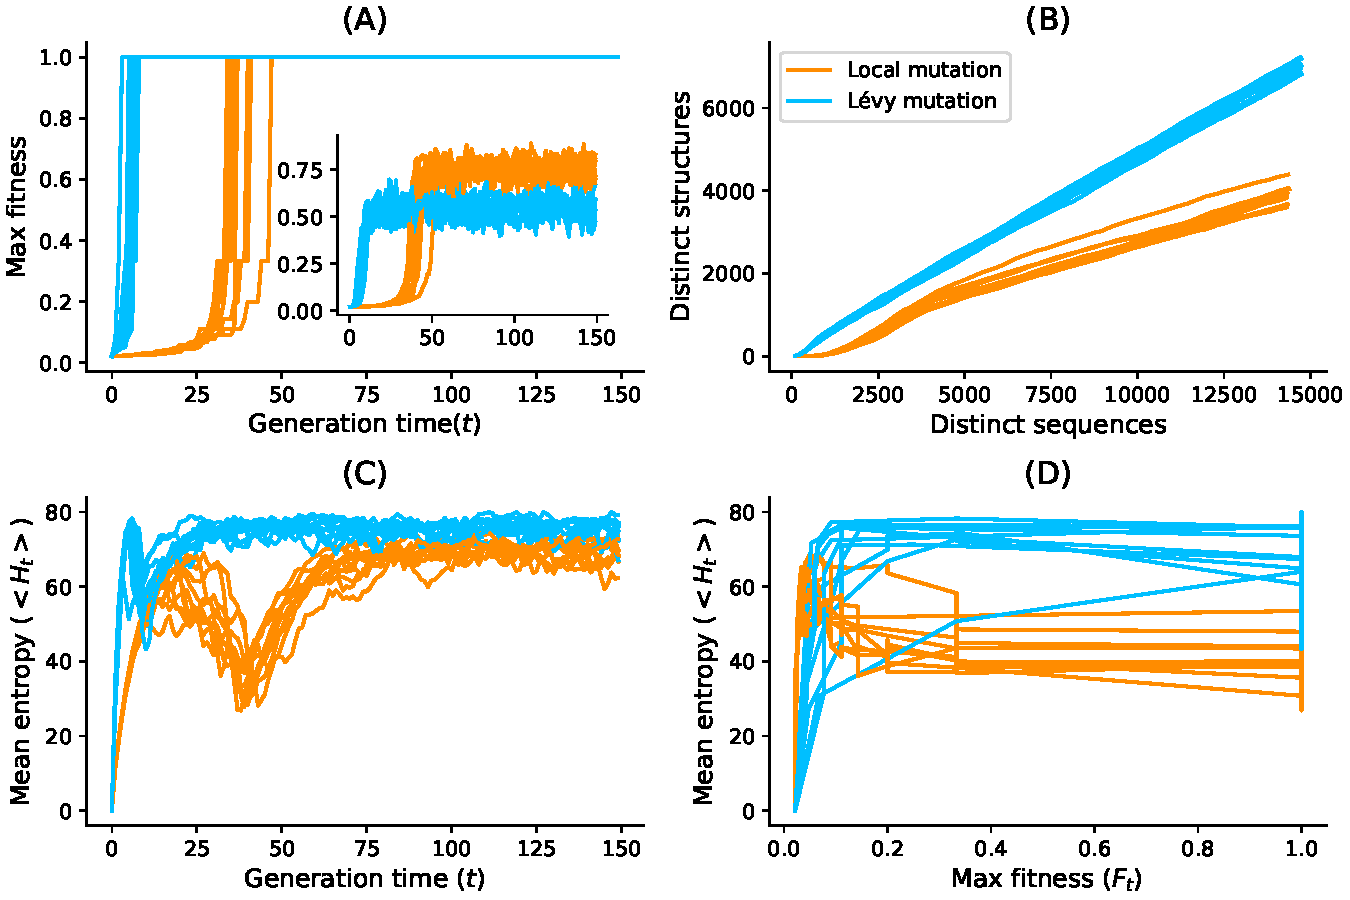
\includegraphics[width=1.0\linewidth]{../res/images/arnaque/fig8.pdf}
	\small 
	\caption{\textbf{Lévy mutation \emph{vs} one-point mutation}. For the \texttt{Eterna100} target structure \texttt{[CloudBeta] 5 Adjacent Stack Multi-Branch Loop}, ten independent runs were performed in which a minimum of $10$ sequences were designed per run.  (A) Max fitness and mean fitness (inset) over time. (B) Distinct sequences \emph{vs.} Distinct structures over time. (C) Mean Shannon entropy of the population sequences over time for both binomial and Lévy mutation. (D) The max fitness plotted against the entropy over time.}
	\label{Fig:diversity}
	
\end{figure}

We argue that the improved performance of the Lévy mutation over local search in target \ac{RNA} structures is due to the high base-pair density of pseudoknotted structures. Given that pseudoknotted \ac{RNA} structures present a higher density of interactions, there are dramatic increases in possible incorrect folds and thus increasing risk of becoming trapped near local optima \cite{hajdin2013accurate}. Large numbers of mutations in paired positions, as implied by a heavy tailed distribution, are necessary to explore radically different solutions. 

To illustrate that Lévy flight performance could be due to base-pair density, we clustered the benchmark datasets into two classes: one cluster for target structures with low base-pair density (density $\leq 0.5$) and a second cluster for structures with high base-pair density (density $> 0.5$). \autoref{Fig:eterna_performance}B showed the number of target sequences available in each low and high density category. The number of targets available in each category are colored according to the percentage of pseudoknot-free targets (\texttt{Eterna100-V1}) vs. targets with pseudoknots (\texttt{Pseudobase++}), showing that pseudoknots are strongly associated with high base-pair densities: $71\%$ of the pseudoknotted target structures have a high base-pair density.  In contrast, the \texttt{Eterna100} dataset without pseudoknots has somewhat higher representation at low base-pair density. If it is true that improved Lévy flight performance is indeed tied to base-pair density, it is possible that similar heavy-tailed mutation schemes could offer a scalable solution to even more complex inverse folding problems. Another measure of difficulty is the length of the target \ac{RNA} secondary structure. When analysing the mean length of the pseudoknot-free targets, the high base-pair density targets are on average $181$ nucleotides longer, and the low-density base-pair targets are $139$ nucleotides (See \autoref{Fig:eterna_performance}C). We have $49$ nucleotides for low-density targets for the pseudoknotted targets and $52$ nucleotides for the high-density targets. That suggests that the Lévy mutation may be a good standard for designing more challenging target structures.

A further effort have been made to understand the cases in which the Levy flight mutation can outperform the Binomial with low mutation rate or a constant one-point mutation rate. The key point of a Lévy mutation for the Inverse folding problem partially may rely on the base-pair density and the stability of stems with budge.  

Although we believe that Lévy flight-type search algorithms offer a valuable alternative to local search, we emphasise that its enhanced performance over say \texttt{antaRNA} is partially influenced by the specific capabilities of existing folding tools. Their limitations may account for the degradation of these tools as the pseudoknot motifs get increasingly complex (i.e. the incapacity of existing folding tools to predict some pseudoknot motifs influences the performance of both \texttt{aRNAque} and \texttt{antaRNA}). The Lévy mutation has also shown less potential in controlling the GC--content of the designed sequence when compared to \texttt{antaRNA} on pseudoknotted target structures. \texttt{antaRNA}'s parameters used in this work were tuned using \texttt{pKiss}; therefore, it could be possible room for improving the benchmark presented here by retuning them using \texttt{IPKnot} or \texttt{HotKnots}.  Another possible limitation is the fact that most target structures were relatively easy to solve (in less than $100$ generations), which possibly allowed local search to perform better than Lévy search in some cases. Further research on more challenging target structures will improve our understanding of which conditions favour local \emph{vs.} Lévy search.


\section{\texttt{RAFFT}, \texttt{aRNAque} and evolutionary dynamics perspectives}\label{sec:evolution}

The \ac{RNA} inverse folding has deep connections with theoretical evolutionary dynamics studies, where the sequence-secondary structure relationship is a popular model for studying the genotype/phenotype maps \cite{greenbury2016genetic,jaeger2001tectorna}. The folding tool usually maps each sequence to a secondary structure, e.g. \texttt{RAFFT} pathways could be used to compute developmental paths from sequence to secondary structure and then use the most dominant structure as the phenotype realization of a genotype \ac{RNA} sequence. Therefore, the two tools we previously introduced have a direct connection with the evolutionary dynamic, where \texttt{aRNAque} simulates the dynamic evolutionary process and \texttt{RAFFT} computes the genotype/phenotype mapping. This section presents some evolutionary dynamics concepts that could be further studied using \texttt{RAFFT} and \texttt{aRNAque}. 


Similar to \acp{EA}, implemented in \texttt{aRNAque}, simulating a dynamic evolutionary process using \ac{RNA} sequence-secondary structure relationship as a model often involves a population of \ac{RNA} sequences to a given target secondary structure. In such a simulation, we need three main ingredients: replication, selection and mutation. These are the fundamental and defining principles of biological systems. The underlying idea is that the genomic material (the blueprint that determines the corresponding secondary structure) in the form of \acp{RNA} is replicated and passed on to the new offspring from generation to generation. An \ac{RNA} individual is then folded into its corresponding secondary structure at each generation. Fitness is then a function that measures how close the realized structure to the target structure is. Therefore, selection results from different types of \ac{RNA} individuals competing with each other. One \ac{RNA} may reproduce faster and out-compete the others. Occasionally, reproduction involves mistakes; these mistakes are termed mutations. Mutations are responsible for generating different \acp{RNA} that can be evaluated in the selection process, thus resulting in biological novelty and diversity.  

Such a simple model gives a unified framework to precisely define and statistically measure evolutionary dynamics concepts such as plasticity, evolvability, epistasis, neutrality, continuity, and modularity. At the molecular level, plasticity is viewed as the capacity of an \ac{RNA} sequence to assume a variety of energetically favourable secondary structures by equilibrating among them at a constant temperature \cite{ancel2000plasticity}. Such concepts have been extensively studied using the \ac{RNA} inverse folding as a toy model. These studies revealed that selection leads to the reduction of plasticity and, therefore, to extreme modularity \cite{ancel2000plasticity}. Another well-studied property of evolution is neutrality which was first introduced by Kimura \cite{kimura1983neutral}, and it suggested that the majority of genotypic changes (or mutations) in evolution are selectively neutral. The attention to Kimura's contention has led to the discovery of neutral networks in the context of genotype-phenotype models for \ac{RNA} secondary structure \cite{schuster1994sequences,reidys1997generic}. Many recent studies \cite{smerlak2019effective, smerlak2021neutral} use the sequence-secondary structure relationship as a toy model for studying neutral evolution. The neutral property of the \ac{RNA} sequence-structure map contributes to a certain extent to the difficulty of the \ac{RNA} design problem (e.g. when the neutral network is dense, this may quickly increase the chance of getting trapped and thus not improving the fitness). This problem is central to many optimization techniques and has already been mentioned in \autoref{ch:review_design}. Trying to avoid such a situation has motivated the choice of the mutation scheme implemented in \texttt{aRNAque}, which is the Lévy mutation.

Another important issue in evolutionary biology concerns the extent to which the history of life has proceeded gradually or has been punctuated by discontinuous transitions at the level of phenotypes. Distinguishing the notion of continuous from discontinuous changes at the level of phenotypes requires a notion of nearness between phenotypes. This notion was previously introduced by Fontana and Peter \cite{fontana1998continuity}, and it is based on the probability of one phenotype being accessible from another through changes in the genotype. The \ac{RNA} sequence-secondary structure relationship provides a framework where the notion of discontinuity transition is more precise. It allows understanding of how it arises in the model of evolutionary adaptation. This is done by simulating an \ac{RNA} population that evolves toward a \ac{tRNA} target secondary structure in a flow reactor logistically constrained to a capacity of $1000$ sequences. Once the secondary target structure is found, the evolutionary trajectory is backtracked to identify all the distinct structures involved and the transitions between them. An example of a continuous transition in Appendix (see \autoref{fig:contiuity}) is the transition  $18 \rightarrow 10$ whereas the transition $15 \rightarrow 22$ is said to be discontinuous. 

The simulation illustrated in \autoref{app:b8} was performed using \texttt{RNAfold}, the folding tool included in the \texttt{ViennaRNA} package. When using \texttt{ViennaRNA}, the plastic ensemble of an \ac{RNA} sequence $\phi$ is often considered to be the suboptimal ensemble structure $\Sigma_{\phi}$ within a user-defined energy range above the \ac{MFE}  at a constant temperature $T$. The \texttt{ViennaRNA} package provides an efficient tool \texttt{RNAsubopt} allowing to compute $\Sigma_{\phi}$.  In a more rigorous implementation of plasticity, each of those structures in the ensemble $\Sigma_{\phi}$ should result from a developmental pathway. Therefore, the environmental changes may induce a change in the developmental path, allowing switching from one structure in the structural ensemble to another. When considering the set of structures produced using \texttt{RAFFT}, each meta-stable structure represents an \ac{RNA} pathway; therefore, this ensemble can be considered a developmental plastic ensemble. Using RAFFT to simulate the evolutionary dynamic model may provide an alternative framework to study evolutionary concepts such as continuity and plasticity. Perhaps, another way of defining a continuous transition ($S_1\rightarrow S_2$) from structure $S_1$ to $S_2$ will be to check if the structure $S_2$ is in the \texttt{RAFFT}'s structure ensemble of the sequence with \ac{MFE} $S_1$. In that wise, we suggest utilizing \texttt{RAFFT} to study and draw a different interpretation of continuous evolutionary transition.

\section{Conclusion}

In sum, the two computational tools introduced in \autoref{ch:rafft} and \autoref{ch:arnaque} have been further examined. Both tools present advantages and limitations, opening doors to further improvements and applications. 

On the one hand, \texttt{RAFFT} predicts fast \ac{RNA} pathways resulting in an ensemble of metastable structures instead of a single \ac{MFE} structure implemented by most traditional methods. The ensemble structures have the advantages of containing some structures of biological relevance and reproducing complete kinetic simulations of known \acp{RNA}. However, the \texttt{RAFFT} method presents some greediness in the choice of stems, does not provide any criterion allowing to choose biological relevant structures from the ensemble produced and does not account for barriers between structures. Despite these limitations, \texttt{RAFFT} offers improvements to the computational times and \ac{RNA} kinetics, and its versatility opens the door to several applications from \ac{RNA} design to \ac{RNA}-\ac{RNA} interaction. 

On the other hand, \texttt{aRNAque} allowed designing \ac{RNA} sequences with higher diversity at a reduced number of evaluations for pseudoknotted target structures. Except for \ac{CPU} time performance on pseudoknotted targets, the success rate performance on both pseudoknot-free and pseudoknotted target structures showed improvements. Despite this, some \texttt{Eterna100} targets remain unsolvable, opening the door to further investigations. We also discussed some \texttt{aRNAque} limitations, such as the influence of the pseudoknot prediction capacities of existing folding tools in the design process and \texttt{aRNAque} potential to control the GC-content. In addition to these two limitations, most pseudoknotted targets were solvable in less than $100$ generations. These limitations contributed to the description of further research directions.

Our results go beyond the computational \ac{RNA} folding and inverse folding; they can be used to study evolutionary dynamics concepts such as continuity and plasticity. Some perspectives have also been discussed.


